
\begin{table*}
\centering
{\small
    \begin{tabular}{|l|l|c|c|c|c|c|c|c|}
    \hline
	\multirow{2}{*}{~}			& \multirow{2}{*}{Approach}		& \multirow{2}{*}{\parbox{1.9cm}{Sleep Interval (seconds)}}	
																						& \multicolumn{3}{c|}{Average Power (mW)}		& \multicolumn{3}{c|}{Recall} 													\\ \cline{4-9}
								&								&						& Steps		& Headbutts	& Transitions	& Steps					& Headbutts					& Transitions 				\\ \hline
	\multirow{14}{*}{\parbox{1.2cm}{Group 1 90\% idle}}	
								& \multirow{5}{*}{Duty Cycling}	& 2						& \multicolumn{3}{c|}{339}				& 94\%					& 57\%						& 97\%						\\ \cline{3-9}
								& 								& 5						& \multicolumn{3}{c|}{217}				& 82\%					& 14\%						& 47\%						\\ \cline{3-9}
								& 								& 10					& \multicolumn{3}{c|}{140}				& 63\%					& 29\%						& 28\%						\\ \cline{3-9}
								& 								& 20					& \multicolumn{3}{c|}{86.3}				& 48\%					& 14\%						& 32\%						\\ \cline{3-9}
								& 								& 30					& \multicolumn{3}{c|}{63.1}				& 31\%					& 7\%						& 12\%						\\ \cline{2-9}
								
								& \multirow{5}{*}{Batching}		& 2						& \multicolumn{3}{c|}{350}				& \multirow{8}{*}{100\%}& \multirow{8}{*}{100\%}	& \multirow{8}{*}{100\%}	\\ \cline{3-6}
								& 								& 5						& \multicolumn{3}{c|}{186}				&						&							&							\\ \cline{3-6}
								& 								& 10					& \multicolumn{3}{c|}{115}				&						&							&							\\ \cline{3-6}
								& 								& 20					& \multicolumn{3}{c|}{80.1}				&						&							&							\\ \cline{3-6}
								& 								& 30					& \multicolumn{3}{c|}{68.3}				&						&							&							\\ \cline{2-6}
								
								& \multicolumn{2}{l|}{Significant Motion}				& \multicolumn{3}{c|}{67.5}				& 						& 							& 							\\ \cline{2-6}
								& \multicolumn{2}{l|}{Simple Configurable Classifier}	& 48.3		& 23.3		& 18.6			& 						& 							& 							\\ \cline{2-6}
								& \multicolumn{2}{l|}{Oracle}							& 41.5		& 21.6		& 16.4			& 						& 							& 							\\ \hline \hline
								
	\multirow{14}{*}{\parbox{1.2cm}{Group 2 50\% idle}}
								& \multirow{5}{*}{Duty Cycling}	& 2						& \multicolumn{3}{c|}{334}				& 92\%					& 74\%						& 90\%						\\ \cline{3-9}
								& 								& 5						& \multicolumn{3}{c|}{243}				& 79\%					& 31\%						& 53\%						\\ \cline{3-9}
								& 								& 10					& \multicolumn{3}{c|}{176}				& 65\%					& 20\%						& 36\%						\\ \cline{3-9}
								& 								& 20					& \multicolumn{3}{c|}{106}				& 33\%					& 5\%						& 10\%						\\ \cline{3-9}
								& 								& 30					& \multicolumn{3}{c|}{80}				& 25\%					& 11\%						& 12\%						\\ \cline{2-9}
								
								& \multirow{5}{*}{Batching}		& 2						& \multicolumn{3}{c|}{350}				& \multirow{8}{*}{100\%}& \multirow{8}{*}{100\%}	& \multirow{8}{*}{100\%}	\\ \cline{3-6}
								& 								& 5						& \multicolumn{3}{c|}{186}				&						&							&							\\ \cline{3-6}
								& 								& 10					& \multicolumn{3}{c|}{115}				&						&							&							\\ \cline{3-6}
								& 								& 20					& \multicolumn{3}{c|}{80.1}				&						&							&							\\ \cline{3-6}
								& 								& 30					& \multicolumn{3}{c|}{68.3}				&						&							&							\\ \cline{2-6}
								
								& \multicolumn{2}{l|}{Significant Motion}				& \multicolumn{3}{c|}{196}				& 						& 							& 							\\ \cline{2-6}
								& \multicolumn{2}{l|}{Simple Configurable Classifier}	& 188		& 45.3		& 43.3			& 						& 							& 							\\ \cline{2-6}
								& \multicolumn{2}{l|}{Oracle}							& 153		& 42.2		& 29.5			& 						& 							& 							\\ \hline \hline

	\multirow{14}{*}{\parbox{1.2cm}{Group 3 10\% idle}}
								& \multirow{5}{*}{Duty Cycling}	& 2						& \multicolumn{3}{c|}{332}				& 89\%					& 47\%						& 89\%						\\ \cline{3-9}
								& 								& 5						& \multicolumn{3}{c|}{257}				& 76\%					& 28\%						& 26\%						\\ \cline{3-9}
								& 								& 10					& \multicolumn{3}{c|}{198}				& 64\%					& 27\%						& 25\%						\\ \cline{3-9}
								& 								& 20					& \multicolumn{3}{c|}{133}				& 42\%					& 19\%						& 19\%						\\ \cline{3-9}
								& 								& 30					& \multicolumn{3}{c|}{99.1}				& 30\%					& 9\%						& 14\%						\\ \cline{2-9}
								
								& \multirow{5}{*}{Batching}		& 2						& \multicolumn{3}{c|}{350}				& \multirow{8}{*}{100\%}& \multirow{8}{*}{100\%}	& \multirow{8}{*}{100\%}	\\ \cline{3-6}
								& 								& 5						& \multicolumn{3}{c|}{186}				&						&							&							\\ \cline{3-6}
								& 								& 10					& \multicolumn{3}{c|}{115}				&						&							&							\\ \cline{3-6}
								& 								& 20					& \multicolumn{3}{c|}{80.1}				&						&							&							\\ \cline{3-6}
								& 								& 30					& \multicolumn{3}{c|}{68.3}				&						&							&							\\ \cline{2-6}
								
								& \multicolumn{2}{l|}{Significant Motion}				& \multicolumn{3}{c|}{318}				& 						& 							& 							\\ \cline{2-6}
								& \multicolumn{2}{l|}{Simple Configurable Classifier}	& 311		& 65.7		& 51.7			& 						& 							& 							\\ \cline{2-6}
								& \multicolumn{2}{l|}{Oracle}							& 266		& 62.9		& 34.9			& 						& 							& 							\\ \hline
    \end{tabular}
}
	\caption{Event recall and average power for synthetic traces.}
	\label{table:summaryRecallPower}
\end{table*}


\section{Results}
\label{sec:results}

In this section we first present the results of experiments conducted
on synthetic traces collected with our robotic testbed.  We then
present results from experiments on a small number of accelerometer
traces collected from human subjects.  Lastly, we show the results
of simulations on audio traces.

\subsection{Synthetic Traces}

In this section we answer the following questions:

\begin{enumerate}
\setlength{\itemsep}{-3pt}  

\item What are the benefits of SCC over Duty Cycling and
  Batching?

\item Is a generic wake-up condition a good solution for multiple 
  applications?

\item How much additional benefit can be obtained from fully
  programmable wake-up conditions?

\item How important is it to let the applications configure
  the processing algorithms' parameters?
  
\end{enumerate}


\subsubsection{SCC vs. Duty Cycling and Batching}

Table~\ref{table:summaryRecallPower} presents the results of replaying
the traces collected from the robot for the sensing configurations
described in the previous section.  For each application, the table
presents average power consumption and activity recall.  Results are
averages across runs of the same group.  All sensing approaches achieved similar
average precision (Headbutts: 89\%, Transitions: 91\%, Walking:
93\%), and we therefore do not include these numbers in the table.

As expected, Duty Cycling performs poorly.  Short sleep intervals
actually result in an increase in power consumption (339 mW compared to an
average of 323 mW to keep the device continuously awake) due to frequent
transitioning between awake and asleep states.  Longer sleep interval
are more effective at saving energy, but they do so by sacrificing
recall.  For example, a sleep interval of 10 seconds reduces the
Headbutts and Transitions recall bellow 30\%.

Batching achieves perfect recall, but requires long
batching intervals to achieve large energy savings.  Therefore, this
approach is not appropriate for applications with timeliness
constrains.  For example, the user of a gesture recognition
application~\cite{liu2009uwave,schlomer2008gesture} would not be
satisfied if the application detects the performed gesture after a
delay of more than a couple of seconds.  We anticipate that in
practice realistic batching intervals are in the order of a few
seconds, depending on the sensor data acquisition rate and the size
of the data buffer.  Additionally, the device often wakes up to find 
out that no 
events occurred in the current batch. We therefore conclude that 
batching will result in significant energy waste for applications 
interested in low frequency events (e.g., gesture recognition, fall 
detection).

SCC can achieve perfect recall while reducing average power consumption
in all scenarios other than step detection
in Group 3, where walking represents 63\% of the trace and the device
experiences little sleep.  SCC performed best when the event
of interest occurs infrequently, reducing power consumption by up to
94\%.  


\subsubsection{SCC vs. Generic Wake-up Condition}

As expected, the power consumption resulting from the use of a 
wake-up condition trigged by significant motion is 
proportional to the amount of activity in the trace.  This approach
achieves power savings comparable to SCC for step detection (the most
common activity), but significantly higher power consumption for
headbutt or transition detection.  Using a generic wake-up condition
would be inefficient for infrequent events of interest.


\subsubsection{SCC vs. Oracle}

By comparing the performance of the SCC approach to Oracle we
observe that for most usage scenarios, the SCC approach
achieves over 90\% of the available power
savings\footnote{$Available\:Savings=Always\:Awake - Oracle$}.
We conclude that a system that allows
custom code offloading to the low-power processor can achieve minimal
additional power savings.


\subsubsection{SCC: Algorithm Parameter Configuration}

Figure~\ref{fig:wucHeadbuttFFTRecallPowerGroup3} uses the Headbutts
application to illustrate the importance of parameter configuration.  
To obtain these results, we varied the value of the threshold used
in the admission control algorithm.  A threshold that is too strict 
causes a significant drop-off in the
achieved recall.  However, a threshold that is too lenient results in
additional power consumption without any extra benefit to recall
because of unnecessary wake-ups.


\begin{figure}[h]
	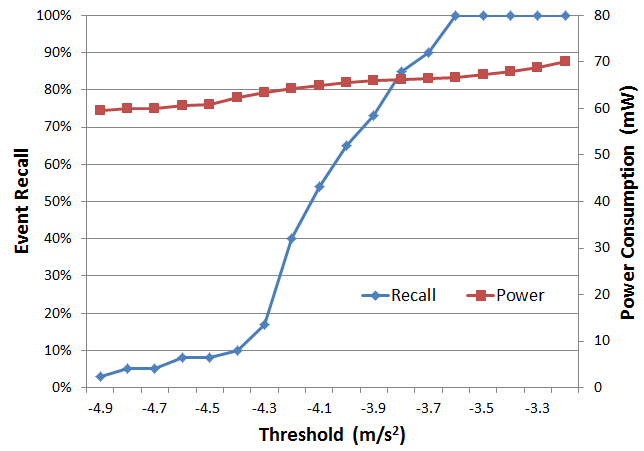
\includegraphics[width=3.1in]{wuc_hb_fft_group3.png}
	\caption{Parameter configuration sensitivity for the Headbutts SCC.}
    \label{fig:wucHeadbuttFFTRecallPowerGroup3}
\end{figure}


\subsection{Human Traces}

\bgroup
\def\arraystretch{1.5}
\begin{table}[t]
\begin{threeparttable}
\centering
{\small
	\begin{tabular}{|l|c|c|c|}
	\hline
	\textbf{Wake-up Mechanism}     & \textbf{Sirens}   & \textbf{Music}   & \textbf{Phrase} \\ \hline
	Oracle                         & 16.8              & 27.2             & 14.7            \\ \hline
	Significant Sound Intensity    & 51.9              & 51.9             & 51.9            \\ \hline
	Simple Configurable Classifier & 63.1\tnote{*}    & 32.3             & 35.6            \\ \hline         
	\end{tabular}
	\begin{tablenotes}
		\item{*} Includes the power consumption of the Stellaris LM4F120H5QR
	\end{tablenotes}
}
\caption{Average power consumption for the audio applications.  Values measured in milliwatts.}
\label{table:macrobenchmarksAudio}
\end{threeparttable}
\end{table}
\egroup

\bgroup
\def\arraystretch{1.5}
\begin{table*}[t]
\centering
{\small
    \begin{tabular}{|l|c|c|c|c|c|c|}
    \hline
	\multirow{3}{*}{\bf Approach}	& \multirow{3}{*}{\parbox{2.1cm}{\bf Sleep Interval (seconds)}}
												& \multicolumn{3}{c|}{\bf Average Power (mW)}
																								& \multirow{3}{*}{\bf Average Recall} \\ \cline{3-5}
									&			& {\bf Trace 1}	& {\bf Trace 2}	&{\bf Trace 3}	& 							\\ 
									&			& 37\% walking	& 22\% walking	& 20\% walking	& \\ \hline
	\multicolumn{2}{|l|}{Always Awake}			& \multicolumn{3}{c|}{323} 						& 100\% \\ \hline
	\multirow{5}{*}{Duty Cycling}	& 2			& 329			& 330			& 330			& 97\%	\\ \cline{2-6}
									& 5			& 272			& 260			& 261			& 92\%	\\ \cline{2-6}
									& 10		& 220			& 195			& 198			& 82\%	\\ \cline{2-6}
									& 20		& 172			& 131			& 134			& 66\%	\\ \cline{2-6}
									& 30		& 148			& 104			& 106			& 57\%	\\ \hline
	\multirow{5}{*}{Batching}		& 2			& \multicolumn{3}{c|}{350} 						& 100\% \\ \cline{2-6}
									& 5			& \multicolumn{3}{c|}{186} 						& 100\% \\ \cline{2-6}
	 								& 10		& \multicolumn{3}{c|}{115} 						& 100\% \\ \cline{2-6}
	 								& 20		& \multicolumn{3}{c|}{80.1} 					& 100\% \\ \cline{2-6}
	 								& 30		& \multicolumn{3}{c|}{68.3} 					& 100\% \\ \hline
	\multicolumn{2}{|l|}{Significant Motion}	& 282			& 157			& 163			& 100\% \\ \hline
	\multicolumn{2}{|l|}{SCC}					& 136			& 77.9			& 72.6			& 100\% \\ \hline
	\multicolumn{2}{|l|}{Oracle}				& 117.8			& 65.8			& 62.3			& 100\% \\ \hline



    \end{tabular}
}
	\caption{Event recall and average power for human traces.}
	\label{table:macrobenchmarksAccel}
\end{table*}
\egroup

Table~\ref{table:macrobenchmarksAccel} shows the results from running the
step detector application on traces collected from three human
subjects.  Since these traces are not annotated with ground truth, we
use the steps detected by a {\em Always Awake} configuration as the baseline for
determining recall.

The results from these experiments show very similar
benefits to the synthetic experiments for runs with low and medium
levels of activity.  For example, the SCC approach achieves
at least 91\% of the available power saving in each of the traces.  

Additionally, we note that the generic wake-up condition performs poorly.  We 
attribute the relatively high power consumption to the fact the human subjects 
were performing a wide range of activities.  While most of the activities were 
not events of interest, they resulted in unnecessary wake-ups.



\subsection{Audio Traces}

Table~\ref{table:macrobenchmarksAudio} shows the average results from running the
the simulations on the collected audio traces.  We omitted the results
for Duty Cycling and Batching because they are similar to the results from
the simulations on accelerometer traces.

For the simulations with a generic wake-up condition, we performed a search
of the parameter space in order to determine the best threshold for sound 
intensity.  The table displays the results for choosing the threshold that
minimizes power consumption, while maintaining 100\% detection recall.
The parameters used in this scenario are over-fitted to the test data, and 
may result in imperfect event recall for different audio traces.  Therefore, 
in practice, a generic wake-up condition such as this one would be more 
lenient (such that it doesn't miss any events of interest), but also consume
more power due to an increased number of unnecessary wake-ups.

SCC performs better than the generic wake-up condition for 2 out of the 3
activities, and nearly matches the power savings of an ideal 
implementation for music detection.  

Due to the higher complexity of the SCC used for siren detection, the more 
powerful Stellaris LM4F120H5QR micro-controller had to be used instead of
the MSP430.  This resulted in an increase in average power consumption by 
more than 40 mW.

For phrase detection, the difference in power consumption between SCC and
the Oracle is attributed to the design of the simple classifier.  The Oracle 
only wakes up when the phrase of interest occurs (<1\% of the trace), while
the SCC is detecting speech segments (5\% of the trace).
